\documentclass{beamer}

\usepackage[utf8]{inputenc}
\usepackage{hyperref}

\usetheme{Berkeley}
\beamertemplatenavigationsymbolsempty
\setbeamertemplate{headline}{}
 
\title{Creating a Workflow in FoodChain-Lab 2}
\date{}
 
\begin{document}
\maketitle
 
\section{1}
\begin{frame}
	\begin{center}
  		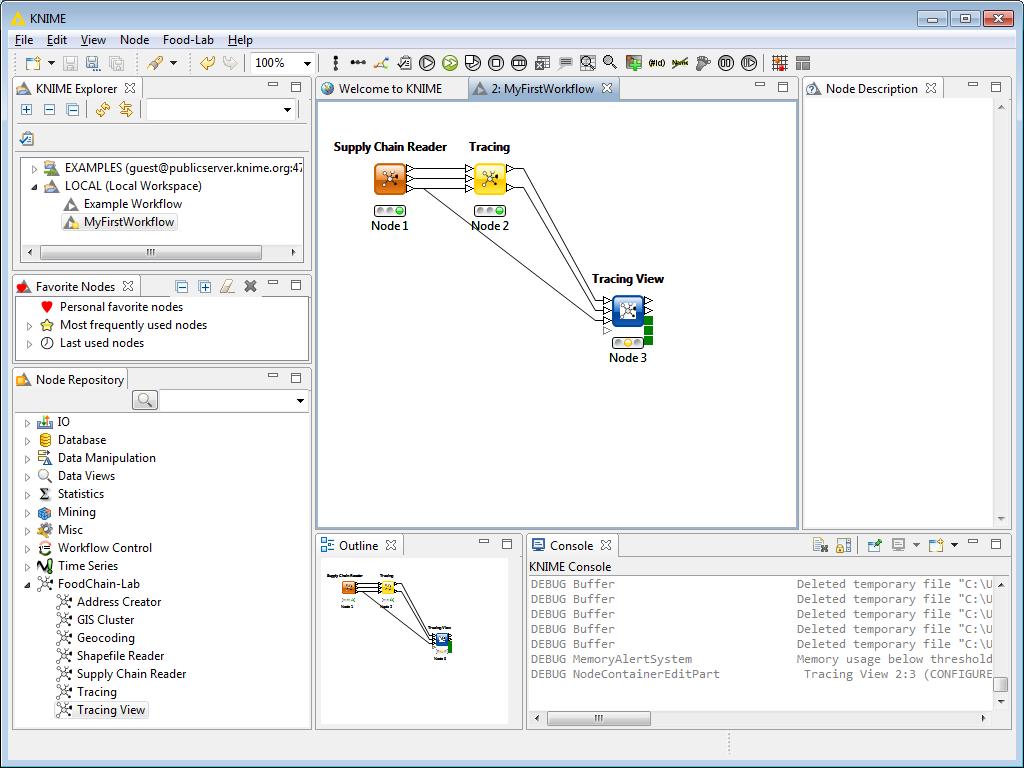
\includegraphics[height=0.6\textheight]{1.png}
	\end{center}
	\begin{itemize}
		\item This is the second part of the tutorial.
		\item You can either do the first part to create this workflow or download it from \url{https://github.com/SiLeBAT/BfROpenLabResources/raw/master/GitHubPages/workflows/My_First_Workflow.zip}.
		\item Double click on the \textbf{Tracing View} to open its dialog.
	\end{itemize}
\end{frame}

\section{2}
\begin{frame}
	\begin{center}
  		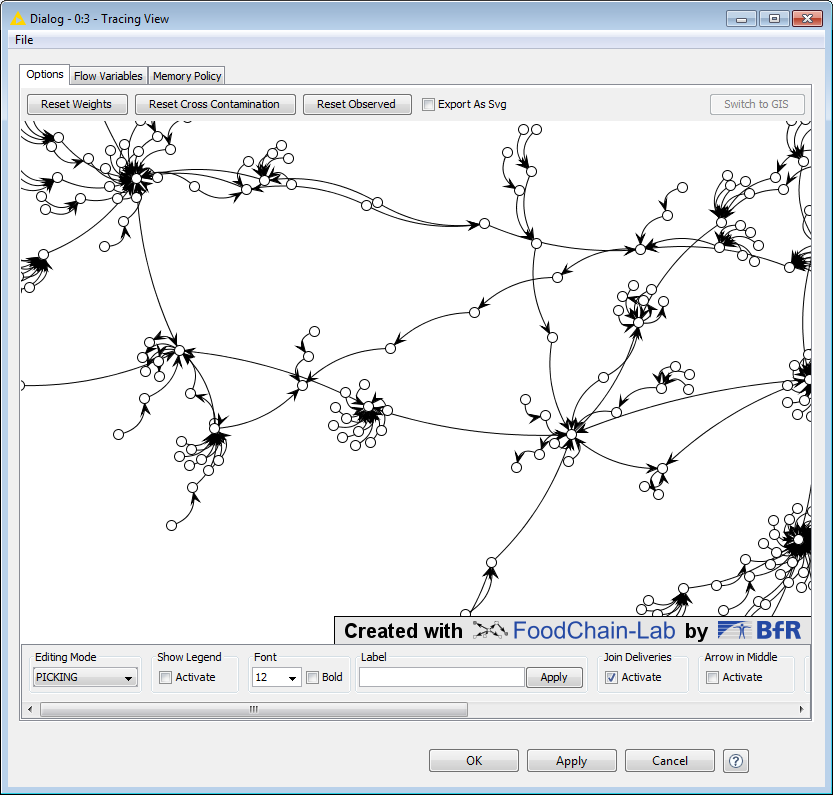
\includegraphics[height=0.6\textheight]{2.png}
	\end{center}
	\begin{itemize}
		\item When you open the \textbf{Tracing View} for the first time, you will notice that the layout process is taking place (stations are moving).
	\end{itemize}
\end{frame}

\section{3}
\begin{frame}
	\begin{center}
  		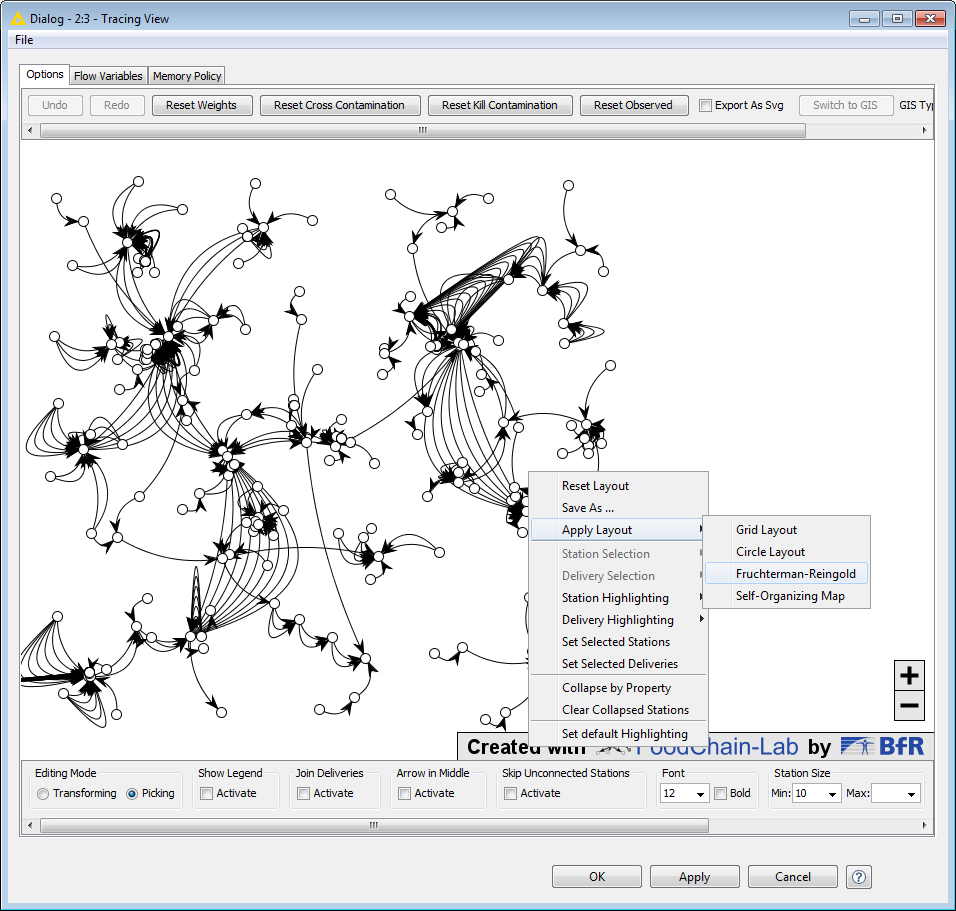
\includegraphics[height=0.6\textheight]{3.png}
	\end{center}
	\begin{itemize}
		\item After the layouting is done, select "TRANSFORMING" as \textbf{Editing Mode} and zoom out till you can see the whole graph (zooming works as in Google Maps).
	\end{itemize}
\end{frame}

\section{4}
\begin{frame}
	\begin{center}
  		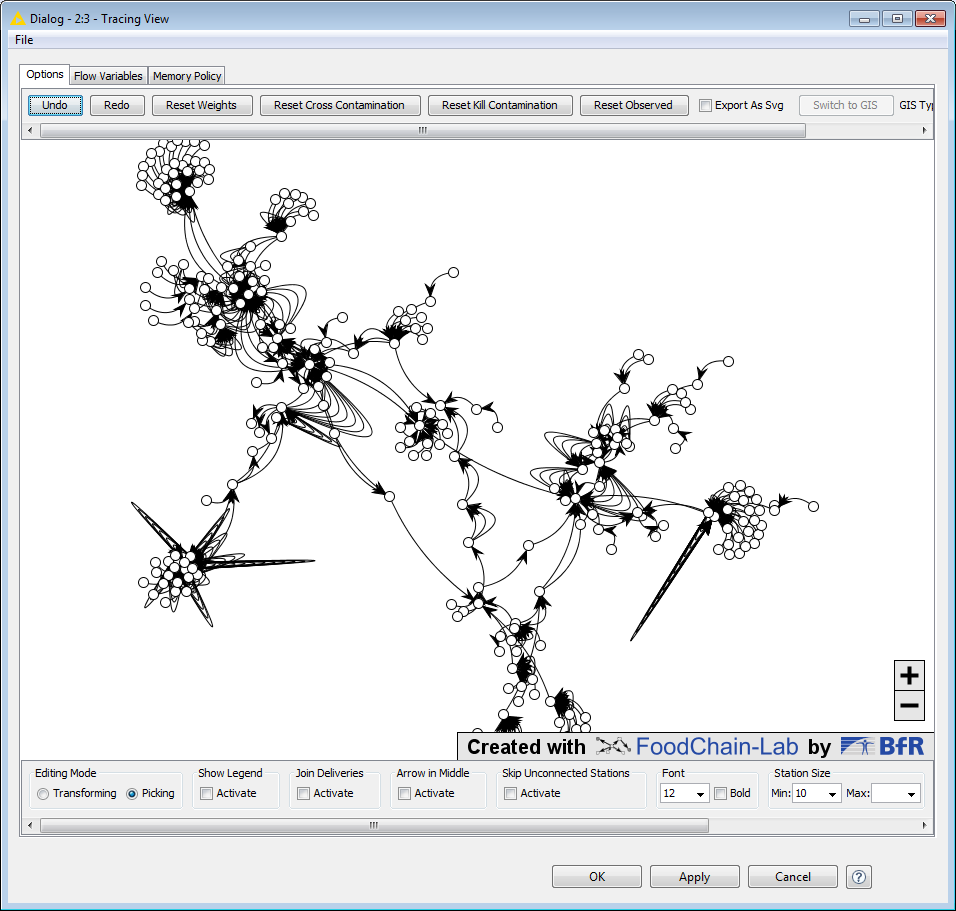
\includegraphics[height=0.6\textheight]{4.png}
	\end{center}
	\begin{itemize}
		\item Right click in the graph to open the context menu and select \textbf{Set default Highlighting}.
		\item Highlighting uses colors and sizes to visualize certain properties of stations/deliveries.
	\end{itemize}
\end{frame}

\section{5}
\begin{frame}
	\begin{center}
  		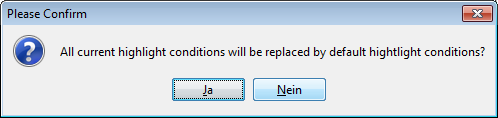
\includegraphics[width=0.9\textwidth]{5.png}
	\end{center}
	\begin{itemize}
		\item In the confirm dialog select \textbf{Yes}.
	\end{itemize}
\end{frame}

\section{6}
\begin{frame}
	\begin{center}
  		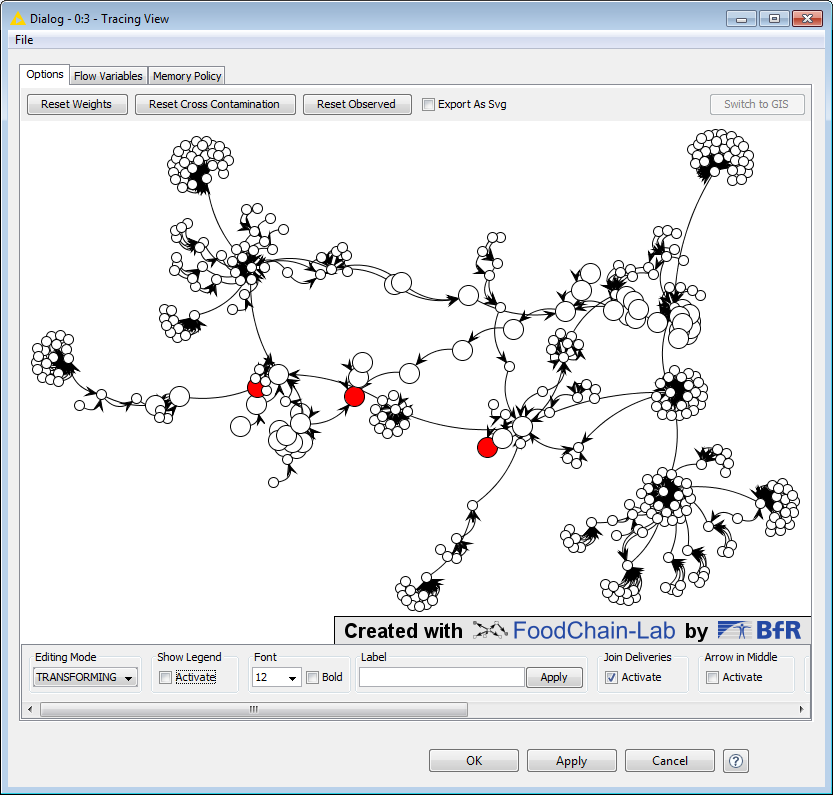
\includegraphics[height=0.6\textheight]{6.png}
	\end{center}
	\begin{itemize}
		\item You will notice, that three stations are colored red now and some stations increased in size.
		\item The red stations are the supermarkets, where set the weight to "1".
		\item The size of each station is based on its "Score".
	\end{itemize}
\end{frame}

\section{7}
\begin{frame}
	\begin{center}
  		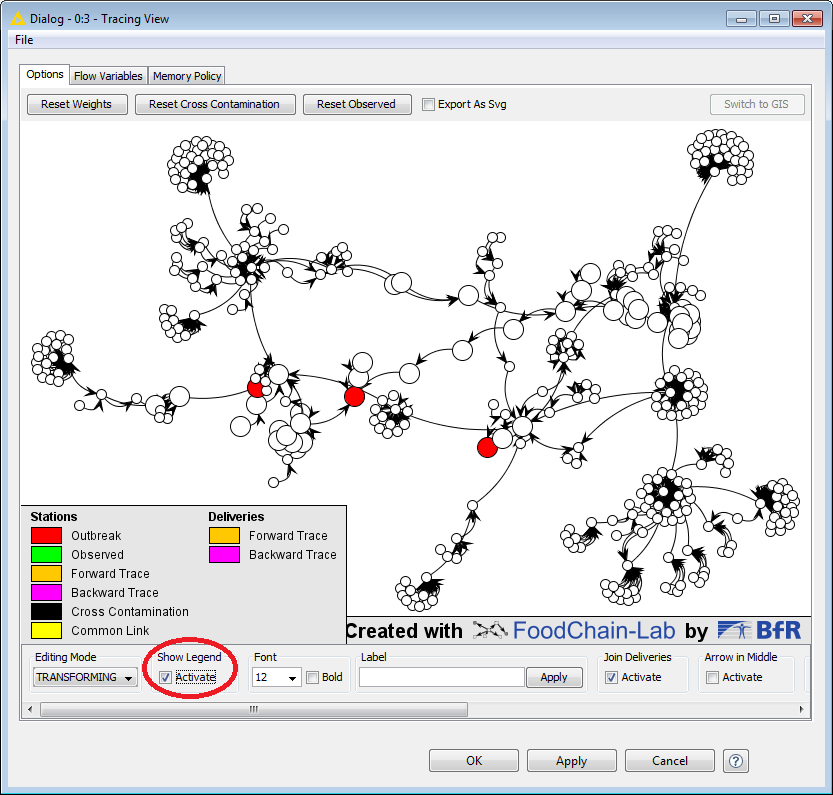
\includegraphics[height=0.6\textheight]{7.png}
	\end{center}
	\begin{itemize}
		\item Activate \textbf{Show Legend} to get a legend for the used colors.
	\end{itemize}
\end{frame}

\section{8}
\begin{frame}
	\begin{center}
  		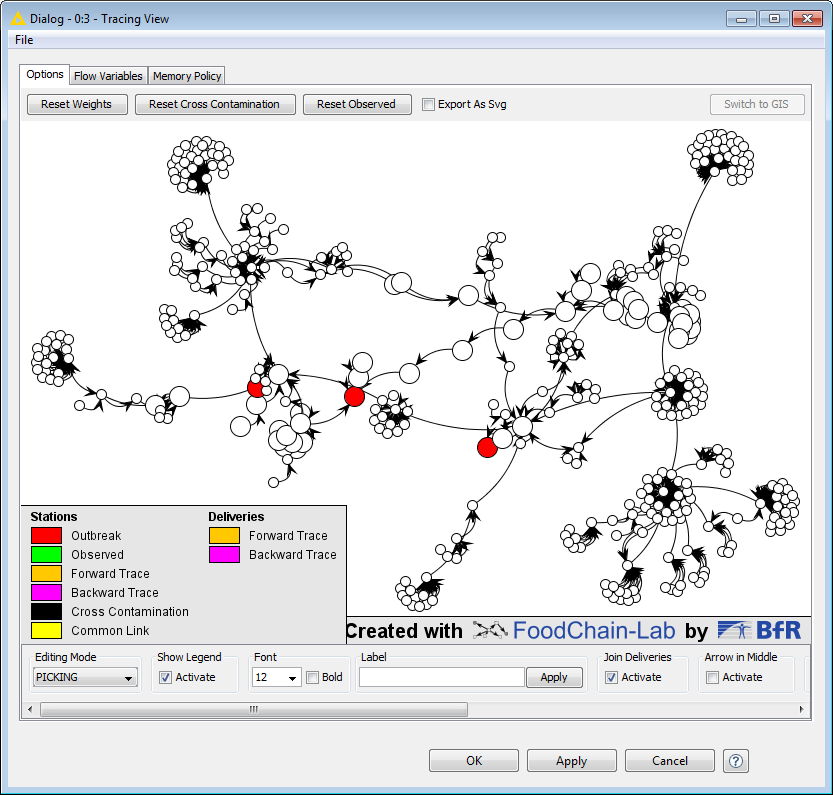
\includegraphics[height=0.6\textheight]{8.png}
	\end{center}
	\begin{itemize}
		\item Now we can obeserve a station to see its delivery trace.
		\item Set "PICKING" as \textbf{Editing Mode} and double click on any station.
		\item We clicked on the station in the red circle.
	\end{itemize}
\end{frame}

\section{9}
\begin{frame}
	\begin{center}
  		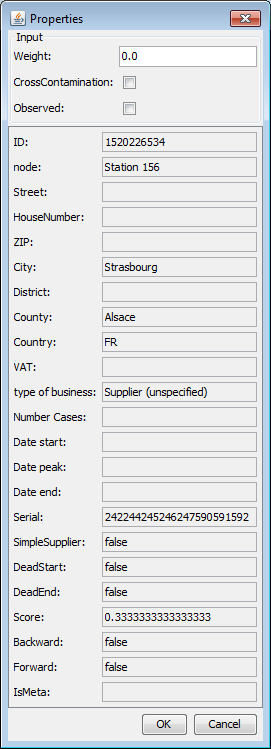
\includegraphics[height=0.6\textheight]{9.png}
	\end{center}
	\begin{itemize}
		\item A dialog will pop up, that all attributes of the station.
		\item Additionally you can change "Weight", "Cross Contamination" and "Observed".		
	\end{itemize}
\end{frame}

\section{10}
\begin{frame}
	\begin{center}
  		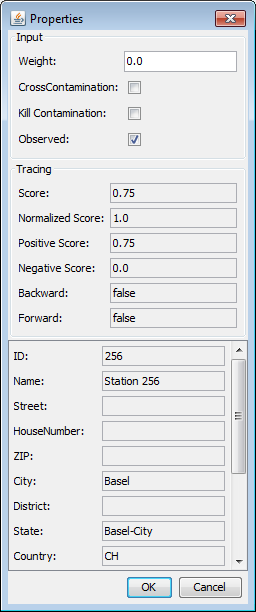
\includegraphics[height=0.6\textheight]{10.png}
	\end{center}
	\begin{itemize}
		\item Select \textbf{Observed} and press \textbf{OK}.
	\end{itemize}
\end{frame}

\section{11}
\begin{frame}
	\begin{center}
  		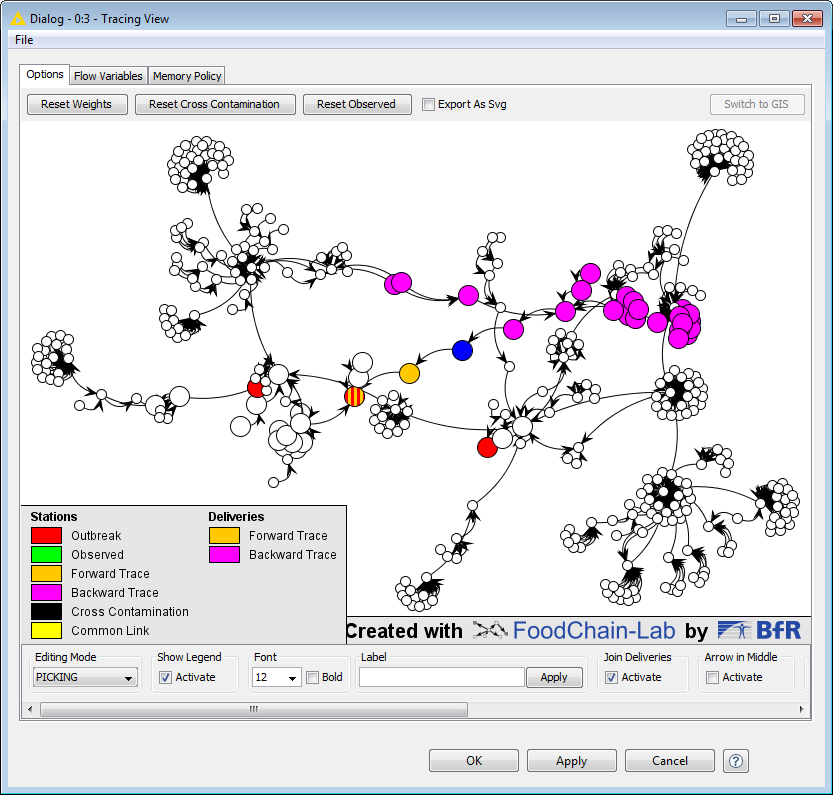
\includegraphics[height=0.6\textheight]{11.png}
	\end{center}
	\begin{itemize}
		\item All stations of the forward trace are orange-colored and the ones of the backward trace are purple.
		\item The deliveries are not colored, since the option \textbf{Join Deliveries} is activated.
	\end{itemize}
\end{frame}

\section{12}
\begin{frame}
	\begin{center}
  		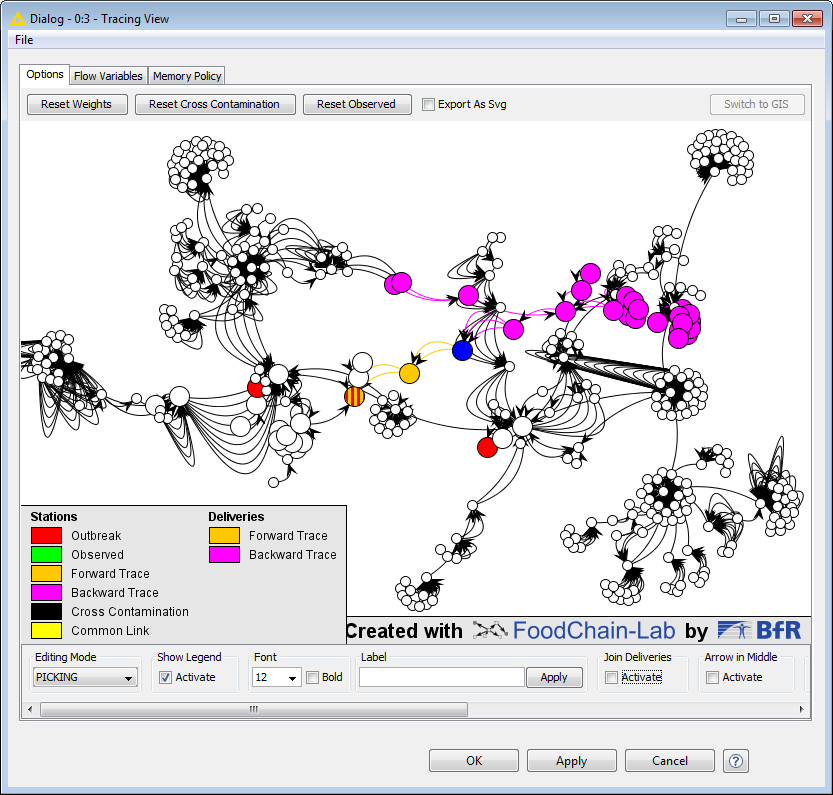
\includegraphics[height=0.6\textheight]{12.png}
	\end{center}
	\begin{itemize}
		\item Deactivate \textbf{Join Deliveries} to see each delivery as a single arrow.
		\item The single deliveries are also colored now, if they are on the forward or backward trace.
	\end{itemize}
\end{frame}

\end{document}